\chapter{Background and Related Work}\label{ch:background-and-related-work}

While Virtual Reality technology has gained more and more traction over the recent years, 30\% to 80\% of users
encounter some form of sickness symptoms during their exposure to virtual environments~\cite{Rebenitsch2016}.
Additionally, these sickness symptoms can have lasting effects after the exposure as well~\cite{LaViola2000}.
The high number of affected users has led to cybersickness being one of, if not the biggest roadblock to a more
widespread adoption of Virtual Reality Devices.

According to LaViola~\cite{LaViola2000} the symptoms of exposure to virtual environments include:
\begin{itemize}
    \item Eye strain
    \item Headache
    \item Pallor
    \item Sweating
    \item Dryness of mouth
    \item Fullness of stomach
    \item Disorientation
    \item Vertigo
    \item Nausea
    \item Vomiting.
\end{itemize}
Vertigo, in the case of VR-sickness particularly benign paroxysmal positional vertigo (BPPV), is a condition where the
individual experiences a false sense of motion, or spinning, and objects or surroundings appear to swirl or
move~\cite{Post2010}.
\\
Several studies also found that severity of symptoms increases with longer exposure times to virtual environments~\cite{Ruddle2004,Min2004,Duzmanska2018}.
However, some studies show that users can adapt, and overall sickness reduces with repeated exposure~\cite{Hill2000}.

Throughout the study of these symptoms, several terms have been used to compound these sickness symptoms that appear
to be similar to the symptoms of motion sickness.
Initially, the term Simulator Sickness was used to describe motion sickness encountered during exposure to flight
simulators~\cite{Saredakis2020}.
The term originated from the assessment of military flight simulators~\cite{Kennedy1993}.
While Simulator Sickness is still used in recent publications, the terms Cybersickness or VR Sickness are generally used
to differentiate, and closer examine the side effects of virtual environments from simulator
sickness~\cite{Saredakis2020,McCauley1992}.
The term VR Sickness specifically is used in discussions and studies about sickness symptoms involving head-mounted
displays (HMD)~\cite{Kim2018,Cobb1999}.
This terminology is often used interchangeably across literature.
The terms Cybersickness and VR Sickness will be used in this study, as Stanney, Kennedy, and
Drexler~\cite{Stanney1997} argue that, while sickness from virtual environments shares many of the symptoms also
experienced during simulator sickness or motion sickness, the sickness profiles are different.
\begin{center}
    \begin{tabular}{ l l l l l}
        \toprule
        \textbf{ } & \textbf{Simulator sickness} & \textbf{Sea sickness} & \textbf{Space sickness} &
        \textbf{Cybersickness} \\
        \midrule
        Highest rating & Oculomotor & Nauseagenic & Nauseagenic & Disorientation \\
        Middle rating & Nauseagenic & Oculomotor & Disorientation & Nauseagenic \\
        Lowest rating & Disorientation & Disorientation & Oculomotor & Oculomotor \\
        \bottomrule
    \end{tabular}
    \captionof{table}{Related conditions symptom profiles according to Rebenitsch and Owen~\cite{Rebenitsch2016}.}
    \label{tab:symptom-profiles}
\end{center}
According to Rebenitsch and Owen~\cite{Rebenitsch2016} cybersickness and other sickness symptoms similar to motion
sickness are polysymptomatic (many symptoms) and polygenic (different manifestation for individuals) and therefore
complex to understand and describe.
To make the sickness and its symptoms easier to survey and examine, Kennedy et al.~\cite{Kennedy1993} categorize the
symptoms listed above into three categories:
\begin{itemize}
    \item Nauseagenic symptoms (dryness of mouth, fullness of stomach, nausea, etc.)
    \item Oculomotor sypmtoms (eye strain, headache, etc.)
    \item Disorientation symptoms (vertigo, dizziness, etc.)
\end{itemize}
The main arguments for the distinction between simulator sickness and cybersickness are that during cybersickness,
disorientation symptoms rank highest and oculomotor symptoms rank lowest, while simulator sickness and traditional
motion sickness usually have the inverted profile, where disorientation symptoms rank lowest~\cite{Stanney1997}.

Cybersickness can also occur without stimulation to the vestibular system, purely through visual cues, unlike motion
and simulator sickness, where stimulation of the vestibular system is needed, but not visual stimulation~\cite{LaViola2000}.
Additionally, Stanney et al.~\cite{Stanney1997} determined that cybersickness can be up to three times more severe
than simulator sickness.
Saredakis et al.~\cite{Saredakis2020} also note significantly higher average Simulator Sickness Questionnaire scores,
although both mention, the scores and questionnaire were established with a focus on military flight simulators used
by military personnel.
While recently, the Simulator Sickness Questionnaire has been adopted to measure cybersickness in virtual
environments, which might be the reason for the higher average scores~\cite{Saredakis2020}.


\section{Common causes of cybersickness}\label{sec:common-causes-of-cybersickness}

Over the recent years there have been several theories trying to explain the sickness symptoms experienced during
extended exposure to virtual environments, especially since the commercialisation of head-mounded virtual reality
devices.
The most common Theories are the sensory conflict theory and the postural instability theory.
Additionally, there are some theories that try to explain why sickness symptoms occur in virtual environments like the
rest frame theory, and the vergence accommodation conflict theory.


\subsection{Sensory conflict theory}\label{subsec:sensory-conflict-theory}

The generally most accepted, and widespread theory is based on a sensory mismatch either between sensory systems of the
body, or between sensory input and expectation given the perceived environment.
Most commonly, a sensory conflict due to vection (the illusion of self movement while stationary) is argued to be the
main cause of cybersickness~\cite{Weech2018,Keshavarz2019}.
Although, other studies like Palmisano, Mursic, and Kim~\cite{Palmisano2017} suggest, that vection is neither the
sole, nor primary source of sensory conflict.
Sensory conflicts like vection can also occur outside virtual environments, for example when a person is in a
stationary vehicle while an adjacent vehicle begins to move~\cite{LaViola2000}.

\begin{figure}[h]
    \centering
    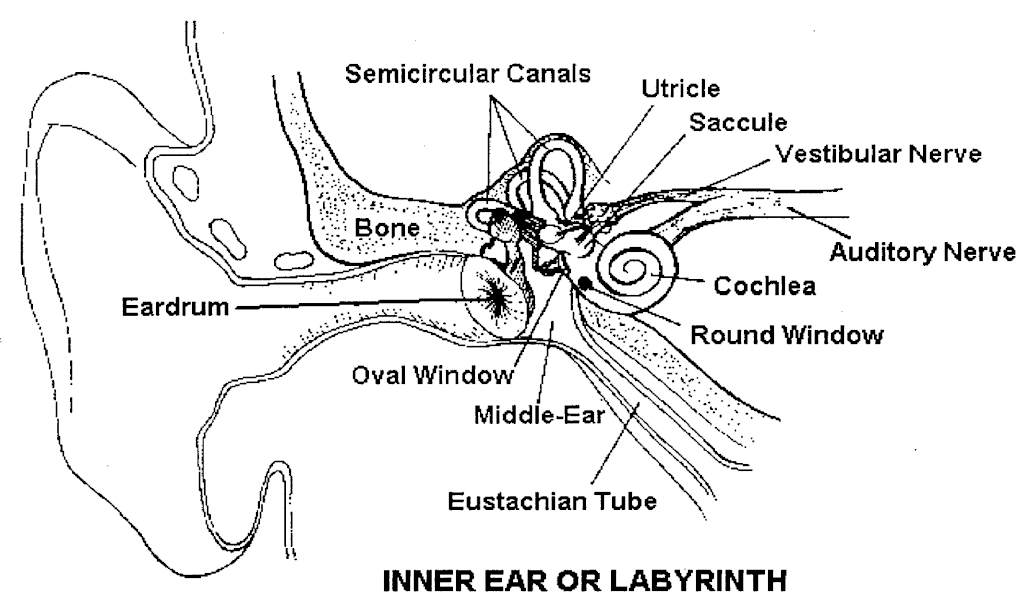
\includegraphics[width=\textwidth]{content/2_related_work/img/VestibularSystem[LaViola2000]}
    \caption{The components of the vestibular system~\cite{LaViola2000}.}
    \label{fig:vestibular-system}
\end{figure}
Important for the sensory conflict theory are visual perception and the vestibular system, shown in
Figure~\ref{fig:vestibular-system}.
The vestibular system consist of the Semicircular Canals to sense angular momentum, and the Utricle and Saccule to
sense linear momentum.
Together, the system functions to compensate for movement, stabilize vision, maintain head posture, and maintain
balance~\cite{Walker2014}.
In virtual environments, the sensory mismatch is usually between the visual system receiving optical flow patterns
characteristic of self motion, while the vestibular system does not perceive these changes in motion.
This sensory conflict lies at the root of simulator sickness and was identified early on, when Barrett and
Thornton~\cite{Barrett1968} noticed that subjects showed simulator sickness symptoms caused by conflict between the
visual presentation of motion and the lack of corresponding vestibular sensation in their fixed-base simulators.
Barrett and Thornton also noticed, that subjects only showed sickness symptoms when the simulator was in a
perspective similar to driving a car, but showed no symptoms when viewing the car from outside, similar to driving a
remote controlled car, as well as passengers showing more severe symptoms than drivers, indicating
that involvement in motion is a factor in the occurrence of simulator sickness~\cite{Tiiro2018,Barrett1968}.

The sensory conflict theory is the most popular theory to explain cybersickness, because it has a steadily growing
amount of studies supporting it, and the theory is intuitive to understand~\cite{Rebenitsch2016,Tiiro2018}.
However, the theory has been criticised by several studies, because sensory conflict theory only states that sickness
is preceded by a sensory conflict, but is unable to predict when cybersickness will occur, or how severe
sickness symptoms will be~\cite{LaViola2000,Rebenitsch2016,Kolasinski1995}.


\subsection{Postural instability theory}\label{subsec:postural-instability-theory}

Another theory for cybersickness symptoms is the postural instability theory proposed by Riccio and Stoffregen~\cite{Riccio1991}.
They found that motion sickness is preceded by periods of postural instability, where small uncontrolled movements and
changes in the subjects centre of gravity occur, and the subject's ability to maintain postural stability is
hindered~\cite{Riccio1991,Clifton2020}.
Stoffregen and Smart~\cite{Stoffregen1998} translated the theory into three predictions:
\begin{itemize}
    \item Experiences of motion sickness are always preceded by increases in postural instability.
    \item Experiences of motion sickness persist until postural stability is restored.
    \item People who are more naturally unstable are more likely to become motion sick during provocative simulation.
\end{itemize}
These predictions have been solidified and are supported by numerous studies on visually induced motion
sickness~\cite{Clifton2020}.
Chardonnet, Mirzaei, and Merienne~\cite{Chardonnet2015}, as well as other studies propose to use the changes in 
range, variance, and frequency of the subject's centre of gravity as a measurement of postural sway.
Based on the accessibility of devices to measure individual's centre of gravity, those measurements have found
increasing popularity in studies to objectively measure subject's postural stability and indicate the potential onset
of cybersickness symptoms~\cite{Lim2020}.
\begin{figure}[h]
    \centering
    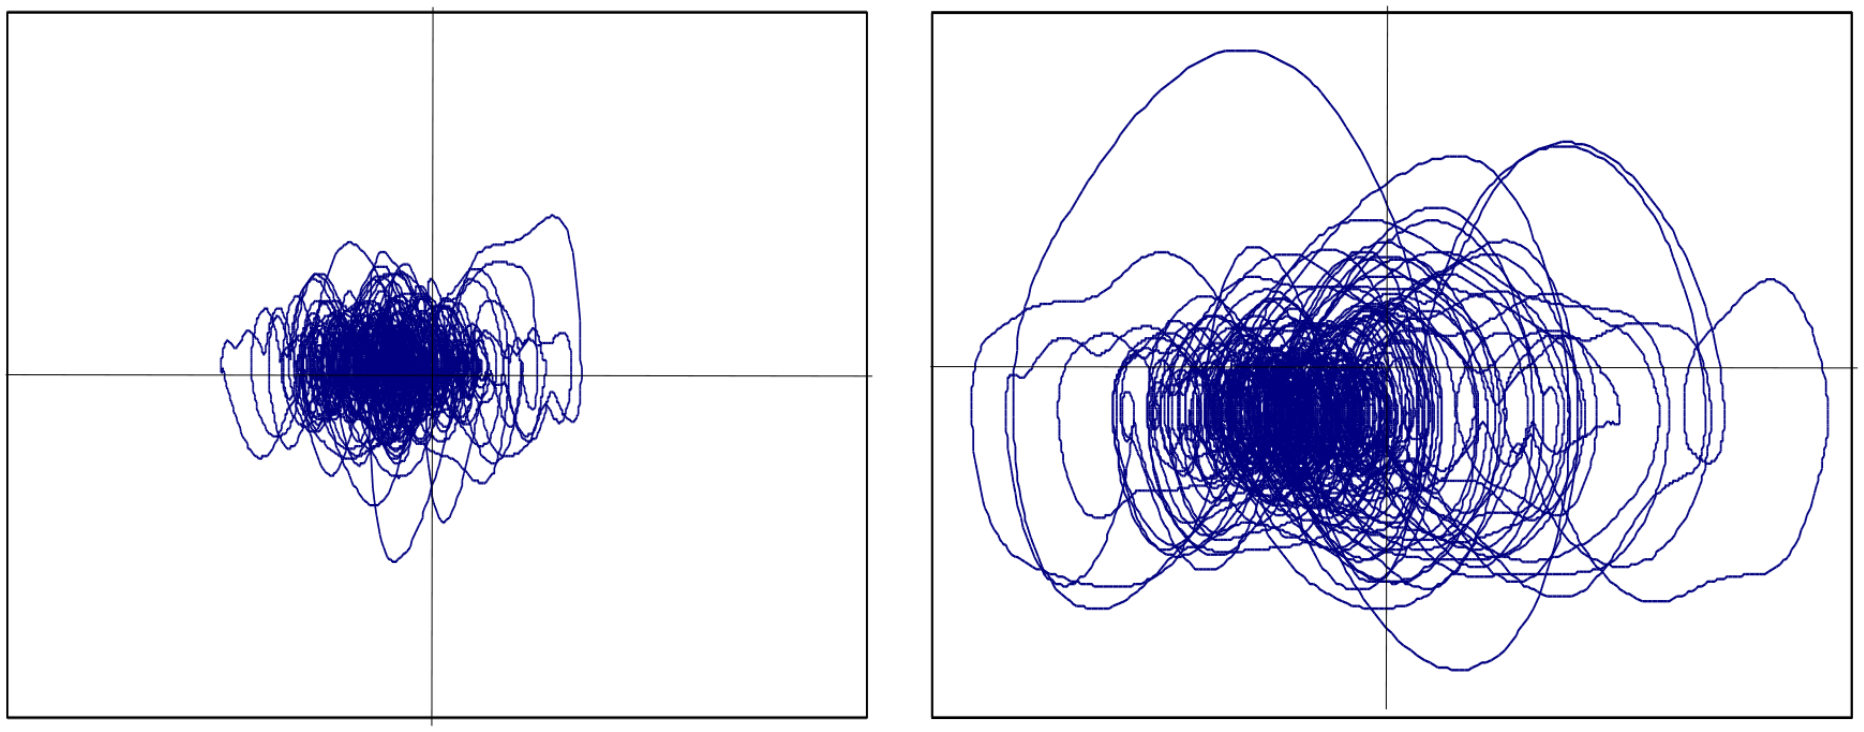
\includegraphics[width=\textwidth]{content/2_related_work/img/PosturalStability[Smart2013]}
    \caption{Comparison of phase portraits (position (in cm) vs. velocity (in cm/s)) for well (left) and sick (right)
        subjects in a dataset measuring postural stability~\cite{Smart2013}.}
    \label{fig:postural-instability-sample}
\end{figure}
A comparison between the natural postural sway of a subject compared to the postural sway when experiencing motion
sickness is shown in Figure~\ref{fig:postural-instability-sample}.
\begin{figure}[h]
    \centering
    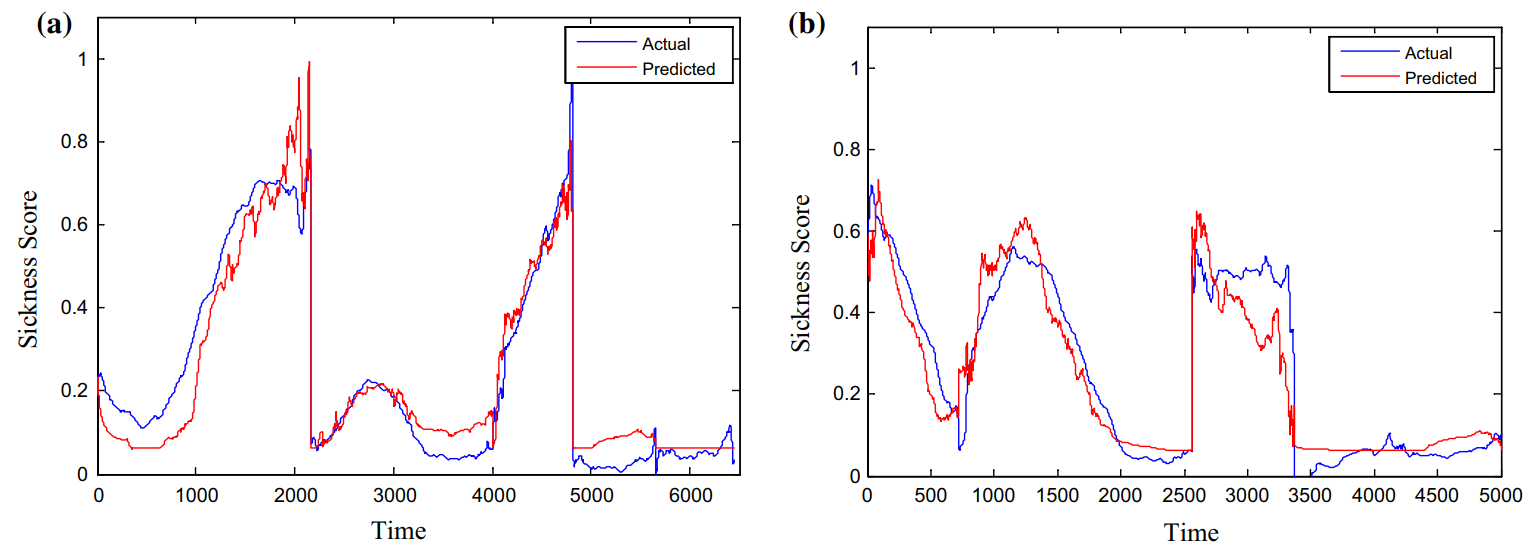
\includegraphics[width=\textwidth]{content/2_related_work/img/PosturalStabilitySicknessPrediction[Lim2020]}
    \caption{Actual sickness (blue) and predicted sickness (red) of (a) training and (b) testing set produced by the
    prediction algorithm by Lim et al.~\cite{Lim2020}.}
    \label{fig:sickness-prediction-algorithm}
\end{figure}
The recent study by Lim et al.~\cite{Lim2020} successfully used postural stability measurements to train an algorithm
to predict VR content's potential to induce cybersickness, as shown in Figure~\ref{fig:sickness-prediction-algorithm},
based on the postural instability theory.


\subsection{Other theories}\label{subsec:other-theories}

\subsubsection{Rest frame theory}
Similar to sensory conflict theory, the rest frame theory argues that a mismatch in sensed gravitation and perceived
up-direction is the cause for sickness symptoms~\cite{Rebenitsch2016}.
\begin{figure}[h]
    \centering
    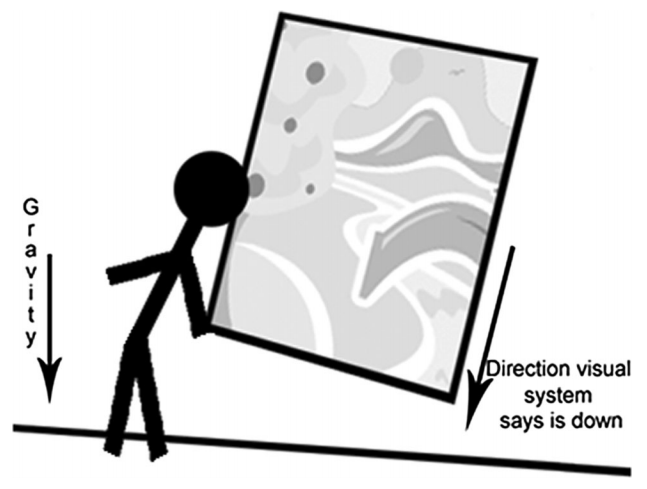
\includegraphics[width=\textwidth/2]{content/2_related_work/img/SensoryMismatchRestFrame[Rebenitsch2016]}
    \caption{Example of sensory mismatch according to rest frame theory~\cite{Rebenitsch2016}.}
    \label{fig:sensory-mismatch-example}
\end{figure}
The rest frame theory also shows similarities to the postural instability theory, as the discrepancy between perceived
up-direction and gravity leads to postural instability and following sickness symptoms~\cite{Rebenitsch2016}.
An example of this sensory mismatch, and resulting postural instability is shown in
Figure~\ref{fig:sensory-mismatch-example}.
The theory also supports the postural instability theory in situations where postural control is lessened, such as in
seated positions where the individual's posture is stabilized.
Several studies like Chang et al.~\cite{Chang2013}, and Duh, Parker, and Furness~\cite{Duh2001b} found, that
superimposing some form of static frame of reference into the virtual environment significantly improves postural
stability and reduces cybersickness symptoms.


\subsubsection{Vergence-accommodation conflict theory}\label{subsubsec:vergence-accommodation-conflict-theory}

Another theory to explain cybersickness symptoms, especially oculomotor symptoms, is the \mbox{vergence-accommodation}
conflict theory.
\begin{figure}[h]
    \centering
    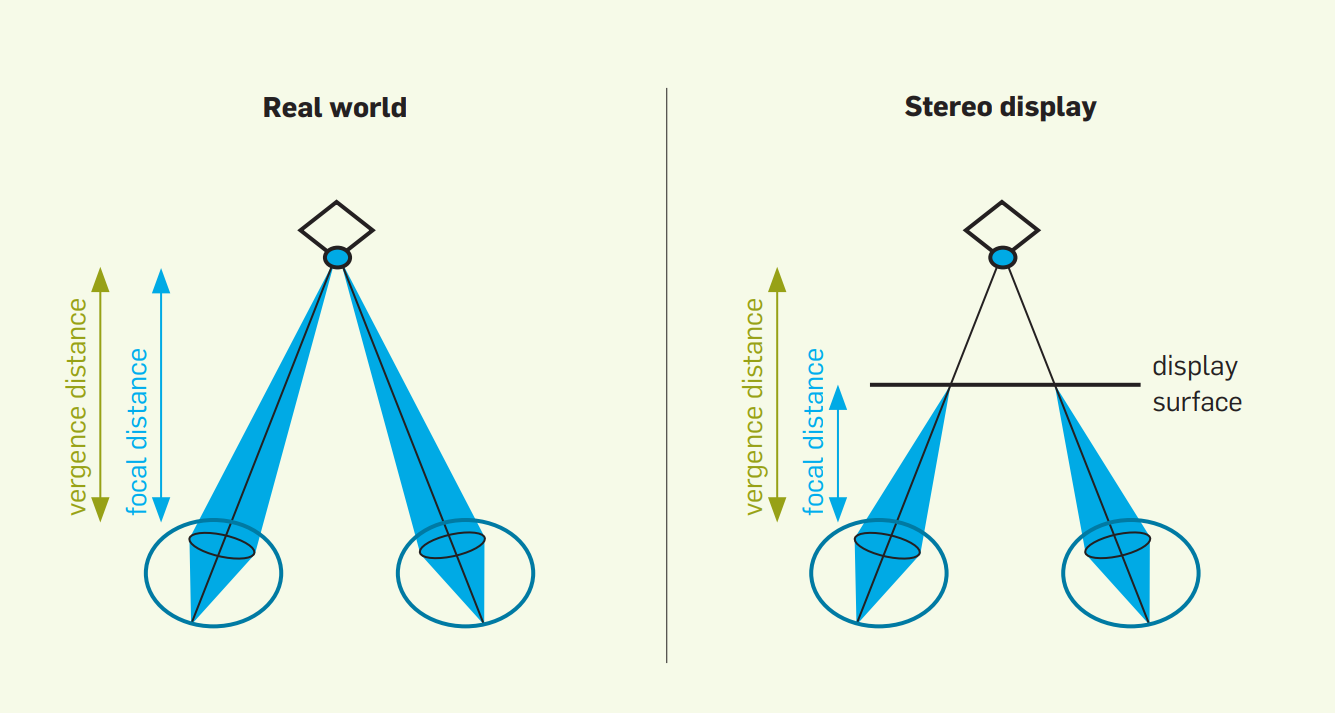
\includegraphics[width=\textwidth/2]{content/2_related_work/img/VergenceAccommodation[Kroeker2010]}
    \caption{Difference between vergence and accomodation distance in the real world (left) and stereoscopic displays
        (right)~\cite{Kroeker2010}.}
    \label{fig:vergence-accommodation-differences}
\end{figure}
Vergence is the simultaneous lateral movement of the eyes when an individual's visual system is adjusting to objects
at different distances~\cite{Kim2014}.
Accommodation is the process of adjusting both eye's focal lengths, focusing on the perceived
object~\cite{Rebenitsch2016}.
In virtual environments, especially in head-mounted displays, images are presented at a fixed screen depth.
This leads to conflict with real life expectations, as vergence and accommodation do not occur naturally at
different distances like in stereoscopic displays~\cite{Saredakis2020}, as shown in
Figure~\ref{fig:vergence-accommodation-differences}.
Kim, Kane, and Banks~\cite{Kim2014} noted that content with high levels of stimulation usually contain more changes
in stimulus distance, and therefore variance of stimulus distance, and level of visual stimulation both increase visual
discomfort and eye strain.


\section{Methods of measurement}\label{sec:methods-of-measurement}

Due to the polysymptomatic and polygenic nature of cybersickness, measurements of cybersickness can prove
difficult, as there is a variety of mostly internal, nonobservable, and subjective symptoms~\cite{McCauley1992}.
Additionally, there can be large individual differences in symptom profiles and susceptibilty, and most symptoms
develop over time and can occur even after the exposure to virtual environments~\cite{McCauley1992}.
Historically, the use of questionnaires is the most popular method of recording occurrences of
cybersickness~\cite{Rebenitsch2016,Saredakis2020}.
The most widely used questionnaire is the Simulator Sickness Questionnaire (SSQ), developed by Kennedy, Lane, Berbaum,
and Lilienthal~\cite{Kennedy1993}.
Recently, several studies have tried refining the SSQ to adapt it for the assessment of virtual reality and
head-mounted displays, resulting in the Virtual Reality Symptom Questionnaire (VRSQ) by Ames, Wolffsohn, and
McBrien~\cite{Ames2005}, and the CyberSickness Questionnaire (CSQ) by Stone III~\cite{Stone2017}.
Another popular questionnaire is the broader formulated Motion Sickness Assessment Questionnaire (MSAQ) by Gianaros,
Muth, Mordkoff, Levine, and Stern~\cite{Gianaros2001}, designed to assess visually-induced motion sickness symptoms
regardless of stimulus context.
In addition to the extensive post-session questionnaires, single item questionnaires like the Fast Motion Sickness
Scale (FMS) by Keshavarz and Hecht~\cite{Keshavarz2011} that are polled in regular intervals during the virtual
environment exposure have gained popularity in cybersickness studies.
Because of the subjective nature of questionnaires, these methods of quantifying cybersickness symptoms have been
criticised and several methods of objective measurement have been researched.
Kim et al.~\cite{Kim2005} studied the changes in sixteen different electrophysiological signals and found several
measurements with a significant positive or negative correlation.
However, these measurements require special equipment that may be unavailable or unintuitive, leading to a low
adoption rate among studies related to cybersickness symptoms and detection.
A more easily accessible method of objective measurement has been measuring the postural stability of individuals
exposed to virtual environments and use the changes in the centre of gravity (CoG) as an indicator for cybersickness
symptoms~\cite{Lim2020}.


\subsection{Subjective Measurements}\label{subsec:subjective-measurements}

\subsubsection{Simulator Sickness Questionnaire}\label{subsubsec:simulator-sickness-questionnaire}

The Simulator Sickness Questionnaire developed by Kennedy, Lane, Berbaum, and Lilienthal~\cite{Kennedy1993} is,
despite being developed in 1993, still one of the most popular methods to measure cybersickness
symptoms~\cite{Saredakis2020}.
Kennedy et al.\ based their developments on the Pensacola Motion Sickness Questionnaire (MSQ), where they identified
several deficiencies that could be improved:
\begin{itemize}
    \item to provide a more valid index of overall simulator sickness severity as distinguished from motion sickness;
    \item to provide subscale scores that are more diagnostic of the locus of simulator sickness in a particular
    simulator for which overall severity was shown to be a problem;
    \item to provide a scoring approach to make monitoring and cumulative tracking relatively straightforward.
\end{itemize}
As part of the last objective, they sought to eliminate the configural approach of the MSQ allowing to automate the
administration and scoring of results.
Additionally, the studies involving the MSQ used differences between post- and pre-exposure scores as their main
indicator, and a pre-exposure checklist where subjects are asked whether they were in other than their "usual state 
of fitness".
Kennedy et al.\ removed both, the two-step approach, and the pre-exposure checklist in an effort to streamline the
administration and scoring process, noting that the SSQ is "intended only for application to post-exposure symptoms,
with the further precondition that a screening of "unhealthy" subjects is required [before exposure]"~\cite[p.
207]{Kennedy1993}.
To tailor the questionnaire to better fit simulator exposure and its sickness symptoms, Kennedy et al.\ eliminated
symptoms that might give misleading indication, were selected too infrequently, or showed no change in frequency or
severity.
Additionally, they sorted the remaining symptoms into separate clusters labeled "Oculomotor" (SSQ-O),
"Disorientation" (SSQ-D), and "Nausea" (SSQ-N).
The distinction allowed to apply a subscale to each cluster, reflecting the impact of simulator exposure on a
different "target system" in the subject.
It also simplified the process of determining where and in what way a simulator may cause problematic
symptoms.
\begin{center}
    \begin{tabular}{ l c c c}
        \toprule
        \textbf{ } & \textbf{ } & \textbf{Weight} & \textbf{ } \\
        \textbf{SSQ Symptom} & \textbf{$N$} & \textbf{$O$} & \textbf{$D$} \\
        \midrule
        General discomfort          & 1 & 1 &   \\
        Fatigue                     &   & 1 &   \\
        Headache                    &   & 1 &   \\
        Eyestrain                   &   & 1 &   \\
        Difficulty focusing         &   & 1 & 1 \\
        Increased salivation        & 1 &   &   \\
        Sweating                    & 1 &   &   \\
        Nausea                      & 1 &   & 1 \\
        Difficulty concentrating    & 1 & 1 &   \\
        Fullness of head            &   &   & 1 \\
        Blurred vision              &   & 1 & 1 \\
        Dizzy (eyes open)           &   &   & 1 \\
        Dizzy (eyes closed)         &   &   & 1 \\
        Vertigo                     &   &   & 1 \\
        Stomach awareness           & 1 &   &   \\
        Burping                     & 1 &   &   \\
        \\
        Total                       & [1] & [2] & [3] \\
        \\
        Score & & & \\
        $N = [1] \times 9.54$ & & & \\
        $O = [2] \times 7.58$ & & & \\
        $D = [3] \times 13.92$ & & & \\
        $TS = [1] + [2] + [3] \times 3.74$ & & & \\
        \bottomrule
    \end{tabular}
    \captionof{table}{SSQ Symptoms and Scoring according to Kennedy et al.~\cite{Kennedy1993}.}
    \label{tab:ssq-scoring}
\end{center}
Table~\ref{tab:ssq-scoring} shows the remaining symptoms and their clustering, as well as the method of scoring the
SSQ as derived by Kennedy et al.
The SSQ symptoms are rated on a four-point scale from 0 to 3, then multiplied by either 1 or 0 (omitted in the table)
according to the weight section of table~\ref{tab:ssq-scoring}, and finally summed up in each column.
The total and subscale scores are then calculated using the formulas in the "Score" section of
table~\ref{tab:ssq-scoring}.
Kennedy et al.\ also mention the possibility to further refine the questionnaire by:
\begin{itemize}
    \item splitting the "Oculomotor" cluster into the disturbance of visual processing (blurred vision, difficulty
    focusing) and the symptoms caused by the disturbance (headache, eyestrain);
    \item splitting the "Nausea" cluster into premonitory signs (increased salivation, burping) and advanced stages
    of nausea (nausea, sweating);
\end{itemize}
As well as moving some symptoms into a "tired and hungry" cluster, believed to be an artifact created by the time
spent during the exposure.
However, Kennedy et al.\ state that there are not enough simulator-relevant symptoms to provide adequate reliability
for smaller clusters, and recommend using the three cluster solution.
Despite the general adoption of the SSQ, there are several problems, especially for the assessment of
cybersickness symptoms in virtual environments, that Kennedy et al.\ recognize in their study.
\begin{center}
    \begin{tabular}{ l l c c c c}
        \toprule
         & & & \textbf{SSQ} & \textbf{Scale M} & \\
        \textbf{Simulator} & \textbf{Aircraft} & \textbf{$N$} & \textbf{$O$} & \textbf{$D$} & \textbf{$TS$*} \\
        \midrule
        2F64C & SH-3   & 14.7 & 20.0 & 12.4 & 18.8 \\
        2F120 & CH-53E & 7.5  & 10.5 & 7.4  & 10.0 \\
        2F121 & CH-53D & 7.2  & 7.2  & 4.0  & 7.5  \\
        2F110 & E-2C   & 7.1  & 13.1 & 6.8  & 10.3 \\
        2E7   & F/A-18 & 6.1  & 5.1  & 6.2  & 6.8  \\
        2F117 & CH-46E & 5.4  & 7.8  & 4.5  & 7.0  \\
        2F87F & P-3C   & 4.5  & 15.2 & 4.3  & 10.5 \\
        2F132 & F/A-18 & 2.7  & 6.1  & 0.6  & 4.2  \\
        2F112 & F-14   & 1.7  & 1.8  & 0.0  & 1.5  \\
              &        &      &      &      &      \\
        M     &        & 7.7  & 10.6 & 6.4  & 9.8  \\
        SD    &        & 15.0 & 15.0 & 15.0 & 15.0 \\
        \bottomrule
        * Total Severity & & & & & \\
    \end{tabular}
    \captionof{table}{SSQ Scale Means by Simulator for the Calibration Sample according to Kennedy et al
    .~\cite{Kennedy1993}.}
    \label{tab:ssq-calibration}
\end{center}
The weights for the scoring functions are derived from 1119 pairs of MSQs collected from 9 simulator sites
shown in table~\ref{tab:ssq-calibration} as a calibration sample.
Therefore, the modal position on the Symptoms or the intermediate sums is no indication for symptomatology with
respect to simulator sickness across simulators in general, as the zero point contains between 40\% and 75\% of the
observations in the calibration dataset.
This also means, the sensitivity is at the upper extremes of the symptomatology range, and the scores should be
compared to the calibration set, in table~\ref{tab:ssq-calibration}, instead of
interpreted on their own~\cite{Kennedy1993}.
Kennedy et al.\ conclude that the results should not be used to distinguish among simulators without problems, but
identify and discriminate problem simulators from those without problems.
Other, more recent studies, like Sevinc and Berkman~\cite{Sevinc2020}, and Rebenitsch and Owen~\cite{Rebenitsch2016},
criticise the usage of the Simulator Sickness Questionnaire because of its complex structure, and development
process, as it involves only a sample of highly trained professionals, and a small amount of simulator experiments,
which both do not comply with the modern day HMD-based virtual environments, and diverse applications
and users~\cite{Sevinc2020}.

\subsubsection{Virtual Reality Symptom Questionnaire}\label{subsubsec:virtual-reality-symptom-questionnaire}

Recent studies like Ames, Wolffsohn, and McBrien~\cite{Ames2005} tried to develop a questionnaire based on the MSQ
and SSQ specifically for the assessment of cybersickness symptoms.
Ames et al.\ note that existing methods like the SSQ do not properly address the ocular symptoms that
contribute to cybersickness symptoms in virtual environments.
Examining existing virtual reality research, they identified 23 symptoms split into two clusters, 12 non-ocular, and
11 ocular symptoms.
Ames et al.\ also decided to expand the symptom response scale to seven options sorted into four
labels: "none" (0), "slight" (1, 2), "moderate" (3, 4), and "severe" (5, 6).
In the development study, they exposed 16 subjects to a stereoscopic video played on a
head-mounted display, and recorded the occurring symptoms with the developed VRSQ in two-minute
intervals immediately after the exposure for a total of six post-exposure examinations.
From the results, they identified 13 symptoms with high item-total correlations, that remain in the final
questionnaire.
While, the "nausea" symptom did not meet the correlation criteria, it was retained for research that might involve
more "dynamic imagery".
However, similar studies, like Stone III~\cite{Stone2017}, criticise the validity of the VRSQ to evaluate
cybersickness, as Ames et al.\ only used video input on a head-mounded display, without any user interaction or input
method, resulting in visual stimulus only, similar to existing studies on visually induced motion sickness, but not
explicitly virtual reality sickness symptoms.
Additionally, Stone III notes concerns about the validity of the psychometric evaluation, and the small sample size
used in the development study.
Davis, Nesbitt, and Nalivaiko~\cite{Davis2014} also note the lack of published studies using the VRSQ as a method to
evaluate cybersickness symptoms in their review on cybersickness literature, while Rebenitsch et al
.~\cite{Rebenitsch2016} do not mention the VRSQ at all.

\subsubsection{CyberSickness Questionnaire}\label{subsubsec:cybersickness-questionnaire}

In his study criticising the VRSQ and SSQ, Stone III~\cite{Stone2017} also proposes an alternative solution to
measure cybersickness symptoms, the CyberSickness Questionnaire (CSQ).
Similar to the method Kennedy et al.\ \cite{Kennedy1993} used to refine the SSQ from the MSQ, they reinterpreted the
results of the SSQ in a cybersickness context.
For this, Stone III selected the symptoms clearly indicating cybersickness:
\begin{itemize}
    \item headache
    \item eyestrain
    \item nausea
    \item blurred vision
    \item dizzy (eyes open)
    \item dizzy (eyes closed)
    \item vertigo
    \item difficulty focusing
    \item fullness of head
\end{itemize}
Additionally, they decided to amalgamate "Severe" and "Moderate" responses from the SSQ\@.
Stone III found a two factor solution by separating the Symptoms into two clusters: "Dizziness" and
"Difficulty focusing".
They also note that the SSQ can still be used to record post-exposure symptoms, while the
scoring can be done using the developed CSQ approach by following these steps:
\begin{enumerate}
    \item Administer the SSQ after the exposure to virtual environments.
    \item Remove the unneccesary symptom items from the collected data.
    \item Combine "Moderate" and "Severe" options for each symptom item, resulting in responses "None" (0), "Slight"
    (1), and "Moderate" (2).
    \item Compute the CSQ factors, similar to the SSQ, by multiplying each symptom item with the weight shown in
    table~\ref{tab:csq-scoring} and adding up the items to form the final scores.
\end{enumerate}
\begin{center}
    \begin{tabular}{ l c c}
        \toprule
        \textbf{} & \textbf{Dizziness} & \textbf{Difficulty focusing} \\
        \midrule
        Headache                & $.50$ & $.$   \\
        Eyestrain               & $.$   & $.58$ \\
        Difficulty focusing     & $.$   & $.89$ \\
        Nausea                  & $.84$ & $.$   \\
        Fullness of head        & $.$   & $.55$ \\
        Blurred vision          & $.$   & $.81$ \\
        Dizziness (eyes open)   & $.89$ & $.$   \\
        Dizziness (eyes closed) & $.99$ & $.$   \\
        Vertigo                 & $.54$ & $.$   \\
        \bottomrule
    \end{tabular}
    \captionof{table}{CSQ nine-item, two-factor model for scoring, according to Stone III~\cite{Stone2017}}
    \label{tab:csq-scoring}
\end{center}
Stone III notes that preliminary evidence, and the comparison of CSQ scores with other established visually-induced
motion sickness scoring methods support the validity of the resulting CyberSickness Questionnaire.
However, they note based on the CSQ scores of their study, 57\% of the 202 participants reported no dizziness and 40\%
reported no difficulty focusing, which implies cybersickness was very low, and the study was not focused
explicitly on inducing cybersickness symptoms.
The review of questionnaires by Sevinc et al.~\cite{Sevinc2020} has tested and approved the validity of the CSQ and
concludes that it is a more accurate method of measuring cybersickness symptoms than the SSQ, as it was developed
with a lager sample size and specifically based on the use of virtual reality applications to induce sickness symptoms.

\subsubsection{Motion Sickness Assessment Questionnaire}\label{subsubsec:motion-sickness-assessment-questionnaire}

Gianaros, Muth, Mordkoff, Levine, and Stern~\cite{Gianaros2001} developed the Motion Sickness Assessment
Questionnaire (MSAQ) with the goal to assess motion sickness across a broad range of contexts.
Similar to other studies developing questionnaires, Gianaros et al.\ recognized the multi-dimensionality of motion
sickness symptoms.
However, they felt sopite-related symptoms, like drowsiness, yawning, and disengagement from the environment, were
underrepresented in existing questionnaires~\cite{Gianaros2001,Graybiel1976}.
Including sopite-related symptoms, Gianaros et al.\ identified four dimensions of motion sickness:
\begin{itemize}
    \item gastrointernal symptoms, like sickness, queasiness, or nausea;
    \item central symptoms, like dizziness, disorientation, lightheadedness, or blurred vision;
    \item peripheral symptoms, like being sweaty, clammy, or hot, or cold sweat;
    \item sopite symptoms, like being annoyed, tired, fatigued, or uneasy.
\end{itemize}
Similar to the SSQ, they designed the MSAQ to be used both, for overall motion sickness scores, and assessment of 
distinct dimensions via subscale scores.
\begin{center}
    \begin{tabular}{l c c c c}
        \toprule
        \textbf{Symptom Item} & \textbf{Gastrointestinal} & \textbf{Central} & \textbf{Peripheral} & \textbf{Sopite} \\
        \midrule
        I felt sick to my stomach  & $.36$ & $.$   & $.$   & $.$   \\
        I felt faint-like          & $.$   & $.45$ & $.$   & $.$   \\
        I felt annoyed/irritated   & $.$   & $.$   & $.$   & $.36$ \\
        I felt sweaty              & $.$   & $.$   & $.27$ & $.$   \\
        I felt queasy              & $.36$ & $.$   & $.$   & $.$   \\
        I felt lightheaded         & $.$   & $.45$ & $.$   & $.$   \\
        I felt drowsy              & $.$   & $.$   & $.$   & $.36$ \\
        I felt clammy/cold sweat   & $.$   & $.$   & $.27$ & $.$   \\
        I felt disoriented         & $.$   & $.45$ & $.$   & $.$   \\
        I felt tired/fatigued      & $.$   & $.$   & $.$   & $.36$ \\
        I felt nauseated           & $.36$ & $.$   & $.$   & $.$   \\
        I felt hot/warm            & $.$   & $.$   & $.27$ & $.$   \\
        I felt dizzy               & $.$   & $.45$ & $.$   & $.$   \\
        I felt like I was spinning & $.$   & $.45$ & $.$   & $.$   \\
        I felt as if I may vomit   & $.36$ & $.$   & $.$   & $.$   \\
        I felt uneasy              & $.$   & $.$   & $.$   & $.36$ \\
        \bottomrule
    \end{tabular}
    \captionof{table}{Symptom items and subscale groups, according to Gianaros et al.~\cite{Gianaros2001}}
    \label{tab:msaq-questions}
\end{center}
The Questionnaire consists of between 16 and 20 symptom questions, with the original 16 questions shown in
table~\ref{tab:msaq-questions}~\cite{Gianaros2001,Sevinc2020}.
Each symptom question is rated on a nine-point scale from 1 (Not at all) to 9 (Severly).
The subscale scores are the sum of the weighted symptom items, multiplied by the weights in the respective columns, and
the total motion sickness score is obtained by the following formula, according to Gianaros et al.:
\begin{itemize}
    \item Overall Motion Sickness Score $= ($ sum of all symptom items (without weights) $) \times 1.44$
\end{itemize}
While, Gianaros et al.\ note that the generated symptoms during their study may stem from a relatively narrow range
of motion sickness contexts, they offer the possibility to modify the questionnaire to more accurately reflect the
multiple dimensions of motion sickness across different motion environments.
Although the development process of the questionnaire was based on visually-induced motion sickness using optokinetic
drums and not virtual reality environments, Sevinc et al.~\cite{Sevinc2020} note in their review on cybersickness
that the Motion Sickness Assessment Questionnaire was used in several virtual reality and simulator studies in the
recent years.
Lastly, Gianaros et al.\ argue that their questionnaire supplies valid descriptors of motion sickness in and for
general population, since the symptom items were generated independently by non-experts during the early phases of
their study.

\subsubsection{Fast Motion Sickness Scale}\label{subsubsec:fast-motion-sickness-scale}

In contrast to the multi-dimensional questionnaires, Keshavarz and Hecht~\cite{Keshavarz2011} proposed and validated
a single-item questionnaire that can be administered during stimulus presentation.
This allows for simple and continuous gathering of motion sickness data during the presentation.
The FMS consists of a verbal rating every minute on a 20-point scale between 0 (no sickness) and 20 (frank sickness),
and primarily measures the two cardinal symptoms in motion sickness: nausea, and general
discomfort~\cite{Keshavarz2011}.
Keshavarz and Hecht explain, they use a 20-point scale to better differentiate among lower
degrees of motion sickness symptoms and capture different states of both well-being and sickness.
They argue the extended scale also helps participants to express their feelings and experience more precisely.
Conversely, Keshavarz and Hecht also note the questionnaire's indifference to the physiological correllates or root
causes of motion sickness, and participants are unable to differentiate between nausea and other precursor symptoms
in their answers.
In their defense, they argue the Fast Motion Sickness Scale is only designed to quantify the subjective impressions
of nausea and general discomfort related to motion sickness, without addressing the underlying symptoms or causes.
\begin{figure}[h]
    \centering
    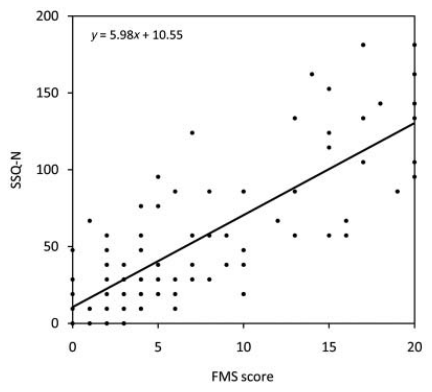
\includegraphics[width=\textwidth/2]{content/2_related_work/img/FMStoSSQcorrelation[Keshavarz2011]}
    \caption{Scatter plot showing the distribution of peak FMS score and SSQ-N subscore for all participants of the
    study by Keshavarz and Hecht~\cite{Keshavarz2011}.}
    \label{fig:fms-ssq-correlation}
\end{figure}
Their validation study showed high correlation between the peak scores of the FMS and the Nausea subscale score of
the Simulator Sickness questionnaire (SSQ-N), as shown in figure~\ref{fig:fms-ssq-correlation}.
Additionally, Rebenitsch and Owen~\cite{Rebenitsch2016} conclude that one-item rating scales are acceptable to
monitor motion sickness symptoms, even though they are not as sensitive or thorough as the multi-dimensional, longer
Questionnaires.
Sevinc and Berkman~\cite{Sevinc2020} also mention a rise in single-item assessment methods, but note that the FMS is
the only version that has been psychometrically evaluated.


\subsection{Objective Measurements}\label{subsec:objective-measurements}

In contrast to the subjective measurements that have been employed in most studies on cybersickness, several studies
have tried linking physiological measurements to the occurrence of cybersickness symptoms in individuals.
Finding reliable physiological cybersickness indicators potentially allows monitoring symptoms without interrupting
the virtual reality exposure through frequent polling of the subject, as used in the FMS, while still generating a
continuous measurement stream to examine symptom development and causes over the duration of the virtual environment
exposure~\cite{Rebenitsch2016}.
One of the broadest studies regarding objective measurements of cybersickness symptoms is the study by
Kim et al.~\cite{Kim2005}, where they collected and tested 16 electrophysiological signals that were used in other
studies as measurements of sickness symptoms in order to find significant correlations indicating a reliable,
objective method measuring cybersickness.
The signals collected before, during, and after the exposure included the following items, which showed a significant
correlation to reported sickness in previous studies:
\begin{itemize}
    \item heart period
    \item respiratory sinus arrhythmia
    \item respiration rate
    \item eyeblink rate
    \item fingertip pulse volume
    \item fingertip temperature
    \item skin conductance
    \item gastric tachyarrhythmia (arrhythmic disruptions of the gastric musculature, often resulting in an upset
    stomach or uneasy feeling)
    \item electroencephalogram (EEG) power spectrum
\end{itemize}
Kim et al.\ used a quite provocative stimulus to test the physiological signals, as 45 out of the 57 subjects
experienced cybersickness symptom during the 9.5 minutes of exposure to virtual environments and subjects reported
cybersickness an average of five times during the exposure.
They also employed a 33-item pre-immersion, and a 49-item post immersion questionnaire to link to better link their
electrophysiological findings to the self-reported levels of cybersickness symptoms experienced.
The questionnaires were compilations of different popular cyber- and motion sickness and susceptibility questionnaires
including the Simulator Sickness Questionnaire.
Kim et al.\ found significant correlations, especially between SSQ scores and gastric tachyarrhythmia, eyeblink rate,
respiration rate, respiration sinus arrhythmia, and heart period.
They found, gastric tachyarrhythmia, skin conductance, respiratory sinus arrhythmia, and relative delta power at F3
and T3 electrode locations of the EEG were significantly higher than the previous recorded baseline.
They also found, heart period, fingertip skin temperature, fingertip pulse volume maximum amplitude, and relative
beta power at F3 and T3 electrode locations were significantly decreased compared to the recorded baseline.
Kim et al.\ suggest that due to the correlation between gastric tachyarrhythmia and cybersickness, the autonomic
nervous system may play a bigger part in the occurrence of cybersickness than previously assumed.
Similar to this study, Roberts and Gallimore~\cite{Roberts2005} found electrogastrogram (EGG) measurements, to detect
gastric tachyarrhythmia, to be a strong indicator of virtual reality exposure and cybersickness symptoms.
Other studies have also used electrocardiogram (ECG) and blood pressure measurements to indicate cybersickness, as 
they found the heart beat becomes stronger, and the blood flow shows lower turbulence during exposure to virtual
environments~\cite{Kiryu2007, Watanabe2008}.

Davis et al.~\cite{Davis2014} note that one detractor to widespread use of physiological measurements may be the
costly hardware and difficulty to analyse the results.
A middle ground has been presented in several studies using measurements of postural stability as an objective, low
cost, and continuous indicator of cybersickness symptoms~\cite{Rebenitsch2016}.
However, Rebenitsch et al.~\cite{Rebenitsch2016} also note that postural sway measurements in many studies are not as
continuous or without the disturbance of the subject as they are often presented, since most measurements require the
subject to enter a specific stance for the measurement.
Most studies use the amplitude, magnitude, and frequency of postural sway to distinguish and predict motion sickness
symptoms, while older studies also examine the time till failure (time until a stance cannot be maintained) or the
stance breaks (number how often the subject fails to maintain a stance) during a specific
timeframe~\cite{Rebenitsch2016}.
Villard, Flanagan, Albanese, and Stoffregen~\cite{Villard2008} and Dong, Stoffregen, and
Yoshida~\cite{Dong2011, Dong2010} both noticed in their studies that subjects who did not experience significant
sickness symptoms had an increased standard deviation of motion during their exposure period, while subjects that
experienced sickness symptoms showed greater variability with smaller average motion compared to the baseline.
Some other studies mentioned similar findings and suggest that subjects may self-adapt to virtual reality exposure by
consciously avoiding head movements when experiencing sickness symptoms~\cite{Rebenitsch2016}.
Another method of low cost, objective measurement of cybersickness is presented by Chardonnet et
al.~\cite{Chardonnet2015}, who found consistent results measuring a subject's centre of gravity (CoG) with a high
correlation to measured SSQ scores.
Lim, Lee, Won, Kala, and Lee~\cite{Lim2020} further extended this measurement, as they proposed to use the VR devices
inertial measurement unit (IMU) to record head dispersion during the exposure period.
They introduced Head Dispersion as a measurement of stability from the following Eq.~\ref{eq:head-dispersion}
\begin{equation}
    \label{eq:head-dispersion}
    Head\ Dispersion = \sqrt{\frac{\sum(roll - \overline{roll})^2 + \sum{(pitch - \overline{pitch})^2}} {n}}
\end{equation}
With the $roll$ and $pitch$ values in degree, and $\overline{roll}$ and $\overline{pitch}$ as the mean values along
the session.
To validate their approach Lim et al.\ compared their IMU sensor data to the centre of gravity sway area measured by an
external sensor as proposed by Chardonnet et al.\ and found high correlation between their measured Head Dispersion
and CoG sway area.
The major advantages of this method are the lack of additional measuring devices needed, and the synchronization
processing, while delivering a continuous indicator of potential sickness symptoms.
However, due to the study's recency, it has not yet seen further adoption or larger sample size studies.


\section{Methods of Mitigation}\label{sec:methods-of-mitigation}

Despite the lack of a definitive cause or widespread adoption of objective measurements to monitor cybersickness
symptoms, several mitigation techniques and best practices have proven effective and have found widespread adpotion
as early as 1992, when McCauley and Sharkey~\cite{McCauley1992} formulated their best practices and recommendations
to prevent and mitigate cybersickness and simulator sickness symptoms:

\textit{Exposure time should be limited until adaption to the VE has occurred}, as some studies found that users
adapt to virtual environments with repeated exposure~\cite{Hill2000}.

\textit{Tasks that require high rates of linear or rotational acceleration should be avoided, or kept brief, until the
individual has fully adapted to the altered environment}, as virtual reality content with high interaction and visual
stimulation tends to lead to more severe experiences of motion sickness~\cite{Saredakis2020}.

\textit{Users of VEs should be considered on an individual basis when determining an adaptation program}.
While this recommendation is focused on adaption programs for simulators, it is also applicable to virtual reality
users, as they show individual differences in cybersickness susceptibility or, for example, preferred locomotion 
method~\cite{Clifton2020}.

\textit{Self-movement through a VE should be at high altitudes above the terrain and/or at lower speeds}, as high
peripharal motion and visual flow are related to cybersickness occurrence and severity~\cite{Buhler2018}.

Additionally, \textit{unusual and extraordinary maneuvers should be avoided in VEs}, as abrupt and counterintuitive
movements can further disorient the user, increasing the risks of cybersickness.

Finally, \textit{users of VE systems should be informed of the possible adverse effects and should be advised to
allow for recovery time after cybertravel before actively engaging in potentially dangerous activities in the real
world, such as driving}, since studies have shown that cybersickness symptoms can occur delayed after the exposure
and have potentially lingering effects~\cite{LaViola2000}.

Apart from these general recommendations, several techniques have found widespread adoption and have shown a positive
impact in mitigating cybersickness symptoms, like the limitation of the Field of View, or the insertion of stable
frames of reference into the virtual scene.


\subsection{Field of View Limitation}\label{subsec:field-of-view-limitation}

The interaction between Field of View (FoV), cybersickness, and the individual's feeling of presence, have been the
subject of many studies, trying to identify the connections and possibly find an optimal solution for the FoV, where
cybersickness symptoms are minimised, while maintaining the feeling of presence as much as possible~\cite{Weech2019}.
Duh et al.~\cite{Duh2001} also found vection to be strongly tied to FoV, as subjects mainly seem to receive
information about vection from their peripheral visual field.
Therefore, a wide FoV causes a greater perception of self-motion, which tends to lead to increased postural
disturbance, and generally resulting in more severe cybersickness symptoms.
Studies like Fernandes and Feiner~\cite{Fernandes2016} recommend to dynamically or at least strategically manipulate
the Field of View in order to reduce visual flow in the peripheral field during periods of high visual flow, reducing
the impact of the resulting vection on cybersickness symptoms.
Duh et al.\ examined the limits of narrow Field of Views and found that, while the experienced motion sickness
increased with higher FoV, there is a significant increase at the 120\textdegree-150\textdegree interval.
Additionally, participants in the study by Lim et al.~\cite{Lim2020} reported "less noticeable" black regions until
the FoV dropped below 60\textdegree.
Lim et al.\ conclude that FoV limitations should be individually adjusted, as users react differently to varying
degrees of FoV limitations, as well as dynamic and fixed FoV limitation.
Finally, they note that, according to their study, dynamic FoV processing and limiting can decrease VR sickness
symptoms by up to 37\%.
